\section{Results and Discussion}\label{sec:Results}

\subsection{The Square Well Potential}

The simple form the square well potential allows us to examine some of the
theoretical discussions, and verify the our implementation of VPA. The
\(S\)-wave phase shift for \(V=-4.0\) MeV found by VPA is shown
in~\cref{fig:squarewell}. As the analytical solution has a modulo
\(\pi\)-ambiguity, we lift the ambiguity by \(k\cot\delta\). The transformed
curves overlap perfectly, validating our solution

\begin{figure}[ht]
  \showthe\columnwidth % Use this to determine the width of the figure.
  \showthe\textwidth % Use this to determine the width of the figure.
  \centering
  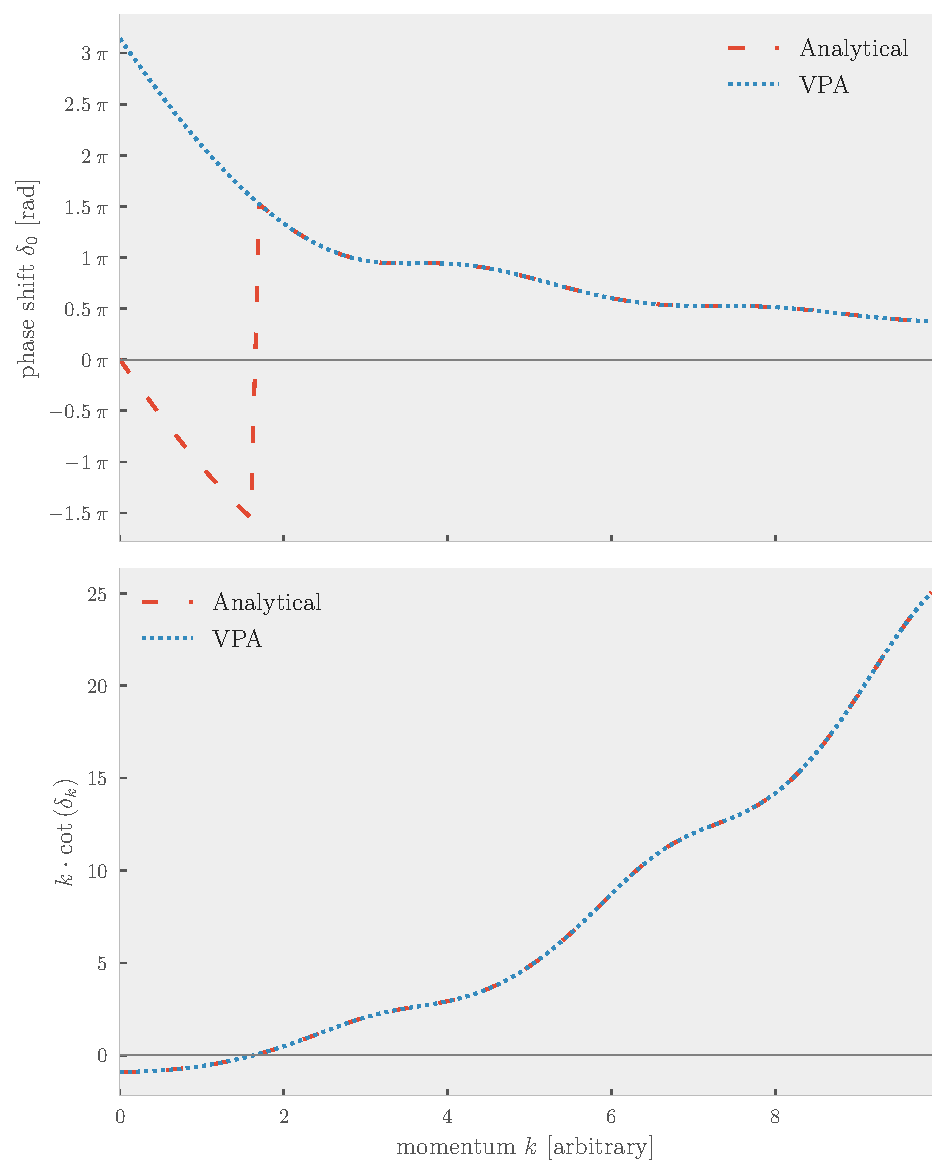
\includegraphics[]{Figures/analytical_cot.pdf}
  \caption{\label{fig:analyticalcot} The S-wave phase shift for a square well
    potential \(V=-4\) MeV, and reduced mass of \(1\) MeV. The \(\pi\)-ambiguity
  in the analytical solution is lifted in the lower panel with the
  transformation \(k\cot{\delta_{0}}\), showing a perfect overlap.}
\end{figure}

The behavior of the square well is next examined by comparing the phase shifts
of the other 
% \begin{figure}[ht]
%   \centering
%   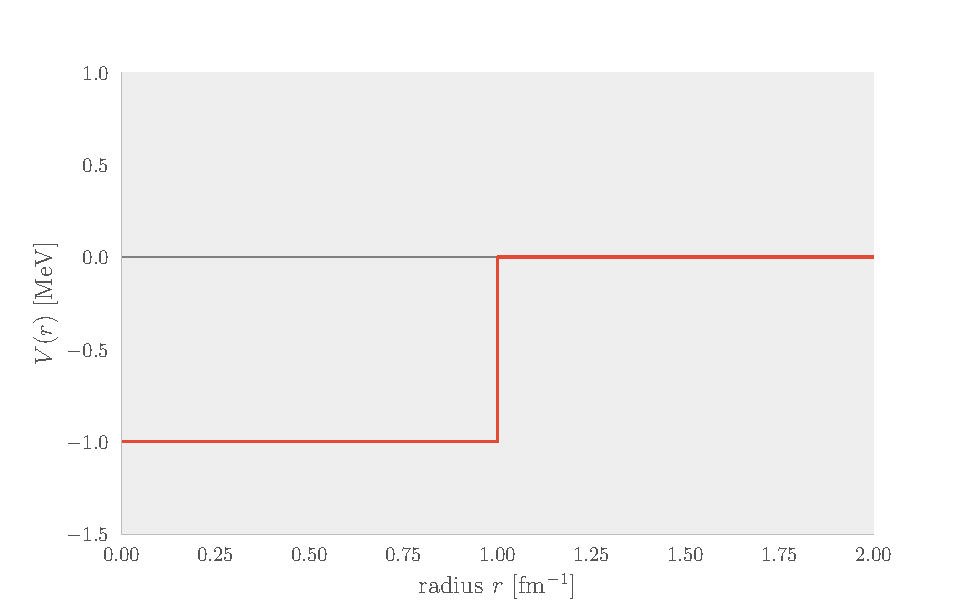
\includegraphics[]{Figures/squarewell.pdf}
%   \caption{\label{fig:squarewell} }
% \end{figure}

\begin{figure}[p]
  \centering
  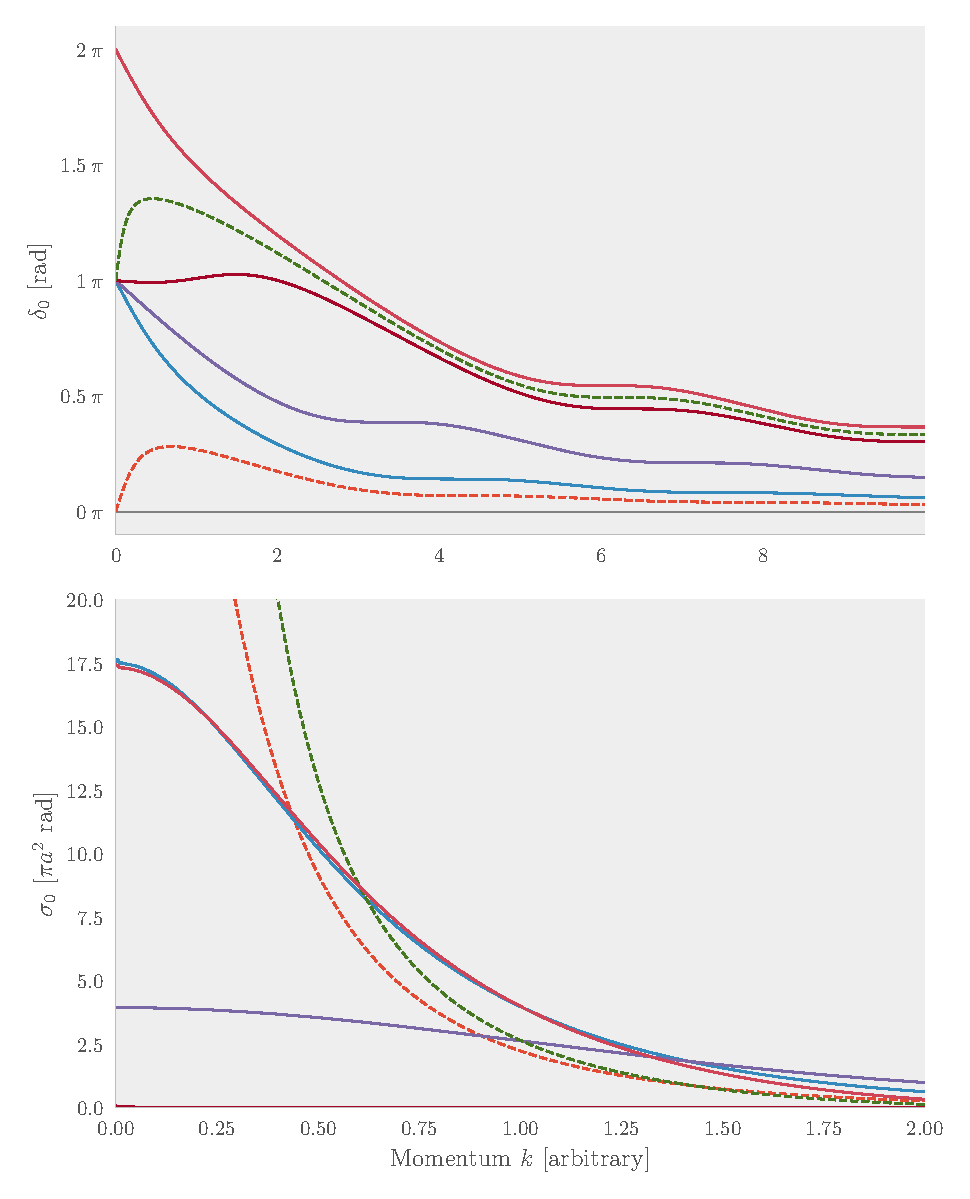
\includegraphics[]{Figures/square_well_wave.pdf}
  \caption{\label{fig:squarewell} }
\end{figure}

\begin{figure}[ht]
  \centering
  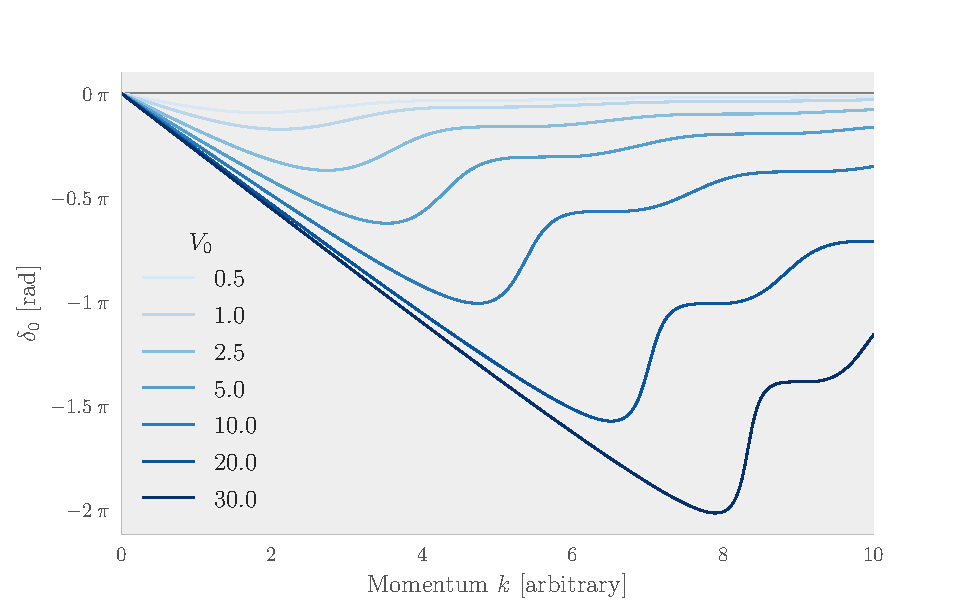
\includegraphics[]{Figures/positive_square_well.pdf}
  \caption{\label{fig:positivesquare} }
\end{figure}


\subsection{The Reid Potential}

\begin{figure}[ht]
  \centering
  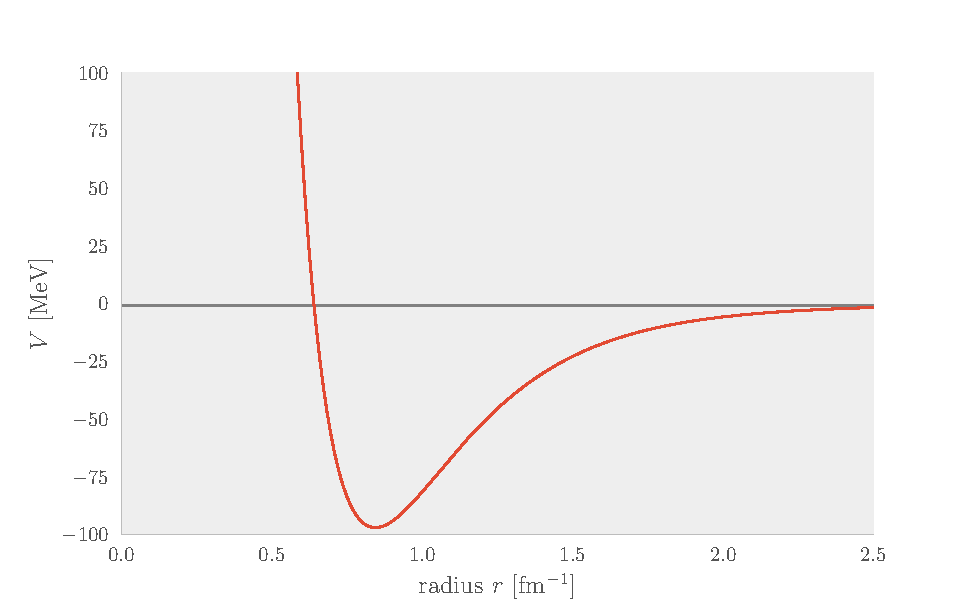
\includegraphics[]{Figures/yukawa.pdf}
  \caption{\label{fig:yukawa} }
\end{figure}

\subsubsection{K-Matrix}
\begin{figure}[ht]
  \centering
  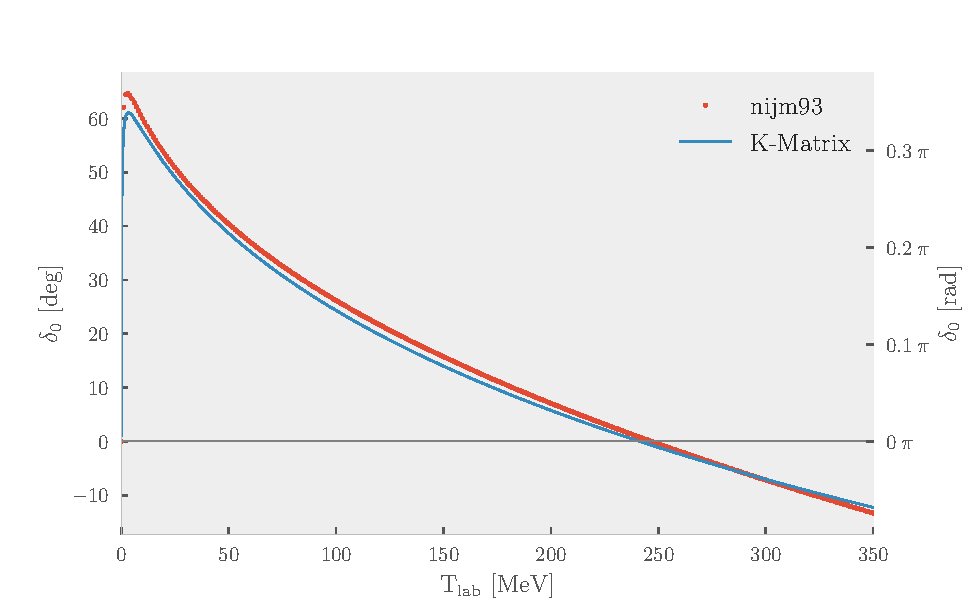
\includegraphics[]{Figures/kmatrix.pdf}
  \caption{\label{fig:kmatrix} }
\end{figure}

\begin{figure}[ht]
  \centering
  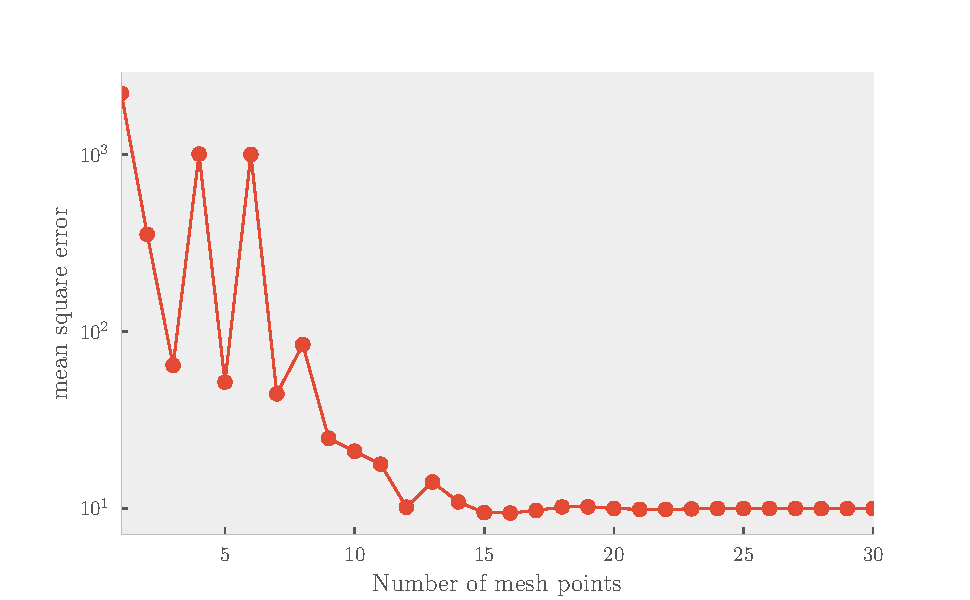
\includegraphics[]{Figures/kmatrix_accuracy}
  \caption{\label{fig:kmatrix_accuracy} The accuracy of the K-Matrix method as a
  function of number of mesh points. For \(n>20\), the error remains near
  constant. 150 phase shifts were calculated for energies \(0\le T_{\text{lab}} \le 150\).}
\end{figure}

\begin{figure}[ht]
  \centering
  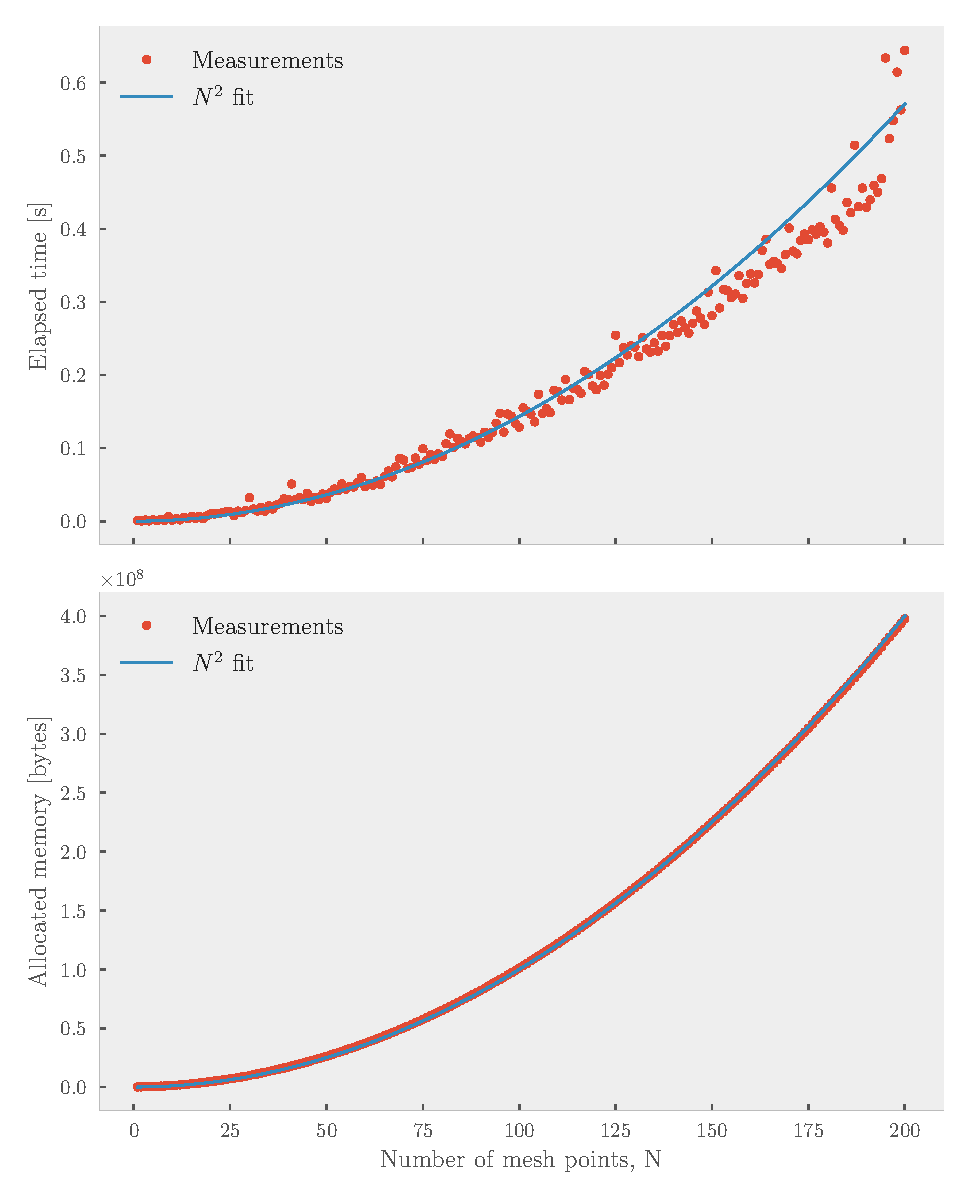
\includegraphics[]{Figures/kmatrix_measurements.pdf}
  \caption{\label{fig:kmatrix_measurements} Resource usage of the K-matrix
    method as a function of number of mesh points. The time shows the median of
    \(10\) repetitions}
\end{figure}



\subsubsection{VPA}

\begin{figure}[ht]
  \centering
  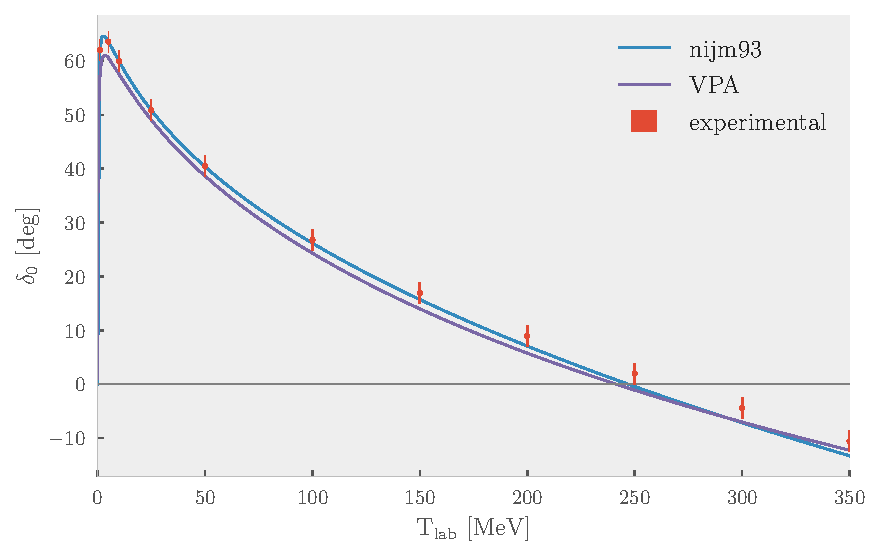
\includegraphics[]{Figures/vpa.pdf}
  \caption{\label{fig:vpa} The resulting \(S\)-wave phase shift from variable
    phase approach}
\end{figure}

\begin{figure}[ht]
  \centering
  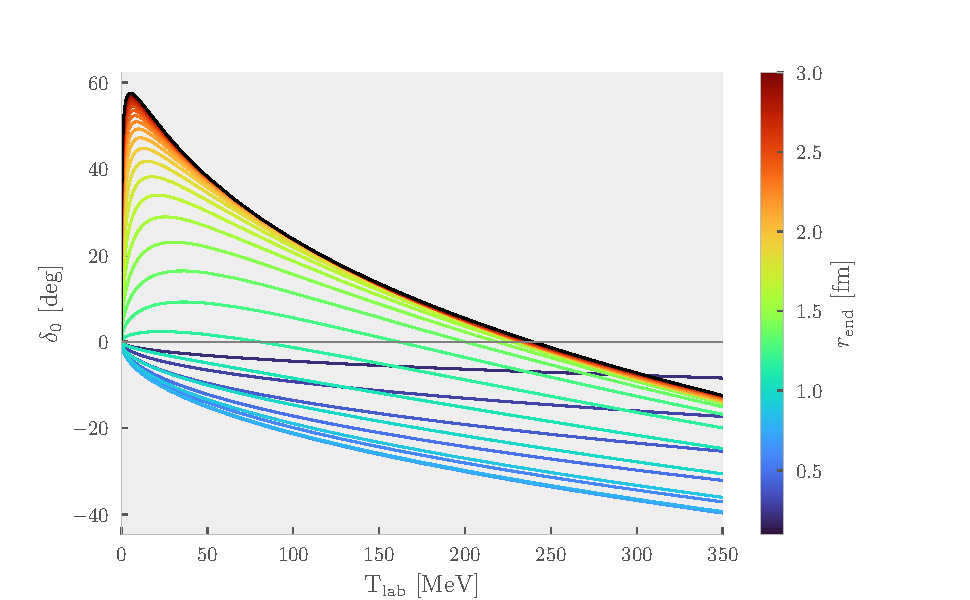
\includegraphics[]{Figures/rend.pdf}
  \caption{\label{fig:rend} The effect of using different cut off points
    \(r_{\mathrm{end}}\) of the potential. Note how the different cut off points
    correspond to the different radii of~\cref{fig:yukawa}.}
\end{figure}



\subsubsection{Comparison}


\begin{figure}[ht]
  \centering
  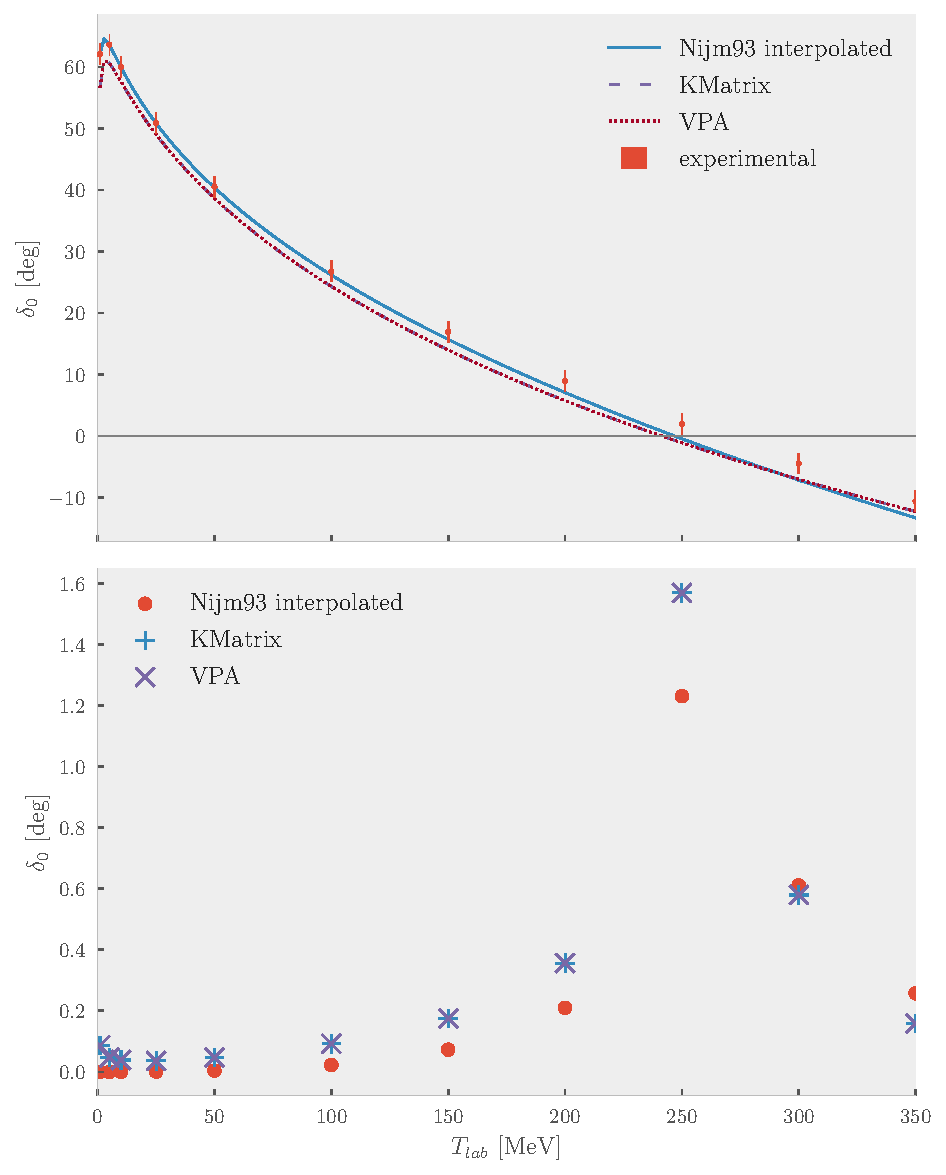
\includegraphics[]{Figures/vpa_kmatrix_compare.pdf}
  \caption{\label{fig:vpa_matrix_compare} The results of K-matrix and VPA using
    good parameters, compared to the \(nijm93\) data. The relative error is
    shown in the lower panel. Only \mbox{\(1 < T_{\mathrm{lab}} < 100\)} MeV are
    included; an arbitrary choice to exclude the jump at \(\approx 0.1 \) MeV
    and the crossing near \(300\) MeV.}
\end{figure}

\begin{figure}[ht]
  \centering
  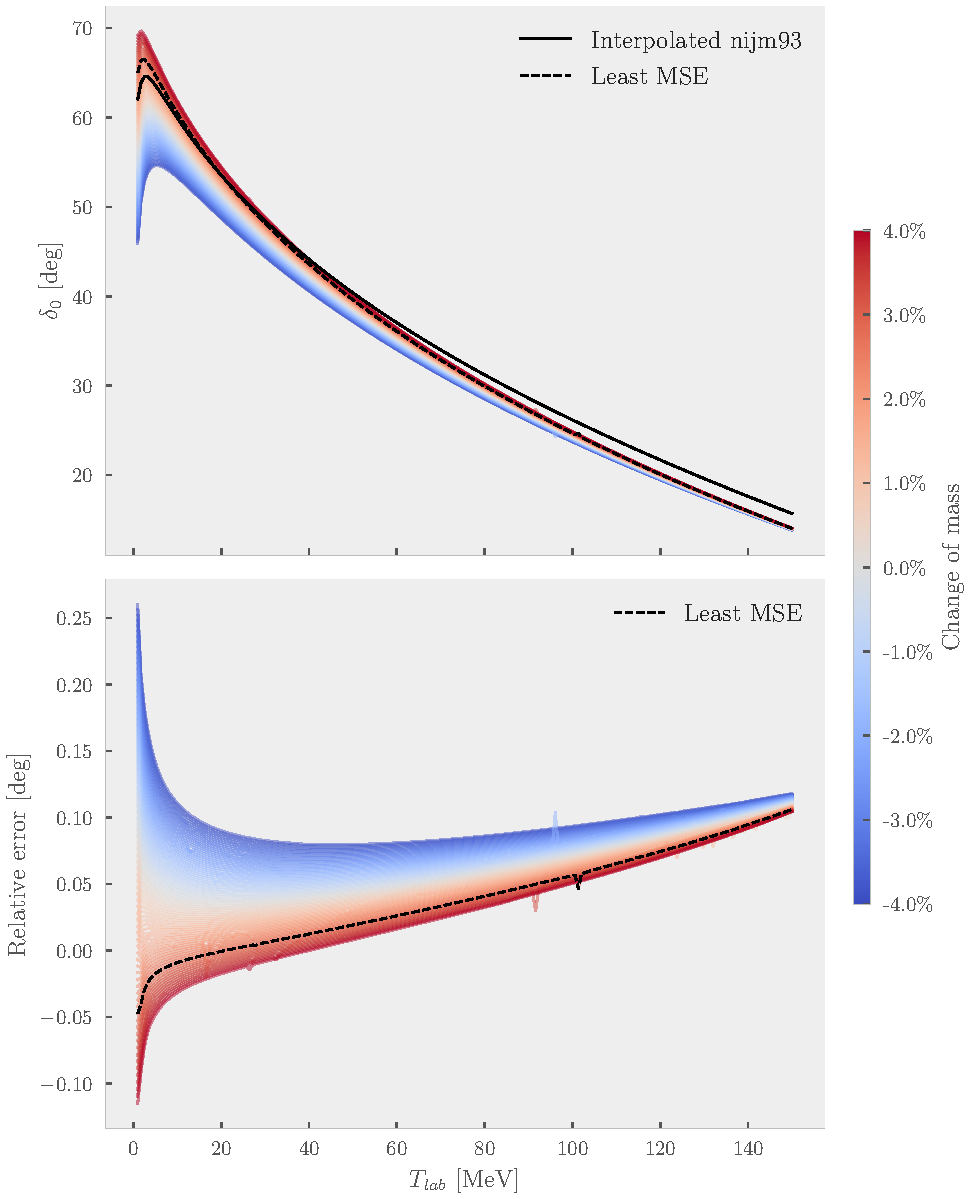
\includegraphics[]{Figures/change_in_mass.pdf}
  \caption{\label{fig:change_in_mass} A linear parameter search using slightly
    different masses ranging from \(96\)\% to \(104\)\% of the original mass.
    The models are compared to \(nijm93\) in the top panel, while the relative
    error to an interpolated version of \(nijm93\) is shown in the bottom panel.
    The model with the mass that gives the minimal MSE is shown as dashed line.
    See the appendix~\cref{fig:optimal_mse} for the MSE curve.}
\end{figure}




%%% Local Variables:
%%% mode: latex
%%% TeX-master: "../main"
%%% TeX-engine: xetex
%%% End:
